\documentclass[a4paper,10pt,english]{article}
\usepackage[utf8]{inputenc}
\usepackage[english]{babel}
\usepackage{
    amsmath,
    graphicx,
    varioref,
    verbatim,
    amsfonts,
    geometry,
    bm
}
\usepackage[usenames,dvipsnames,svgnames,table]{xcolor}
\usepackage[colorlinks=false]{hyperref}

\setlength{\parindent}{0mm}
\setlength{\parskip}{1.5mm}

\definecolor{codegreen}{rgb}{0, 0.6, 0}
\definecolor{codegray}{rgb}{0.5, 0.5, 0.5}
\definecolor{backcolour}{rgb}{0.95, 0.95, 0.92}

\usepackage{listings}

\lstset{
    language=Python,
    backgroundcolor=\color{backcolour},   
    commentstyle=\color{codegreen},
    keywordstyle=\color{magenta},
    numberstyle=\tiny\color{codegray},
    stringstyle=\color{codegreen},
    basicstyle=\ttfamily\footnotesize,
    breakatwhitespace=false,         
    breaklines=true,                 
    captionpos=b,                    
    keepspaces=true,                 
    numbers=left,                    
    numbersep=5pt,                  
    showspaces=false,                
    showstringspaces=false,
    showtabs=false,                  
    tabsize=2,
    breaklines=true,
    morekeywords={assert,None}
}

\title{MEK1100 - Mandatory assignment 2}
\author{William Dugan}

\begin{document}

\maketitle
The full python code can be found at the end of the document.

\begin{figure}[h!]
    \centering
    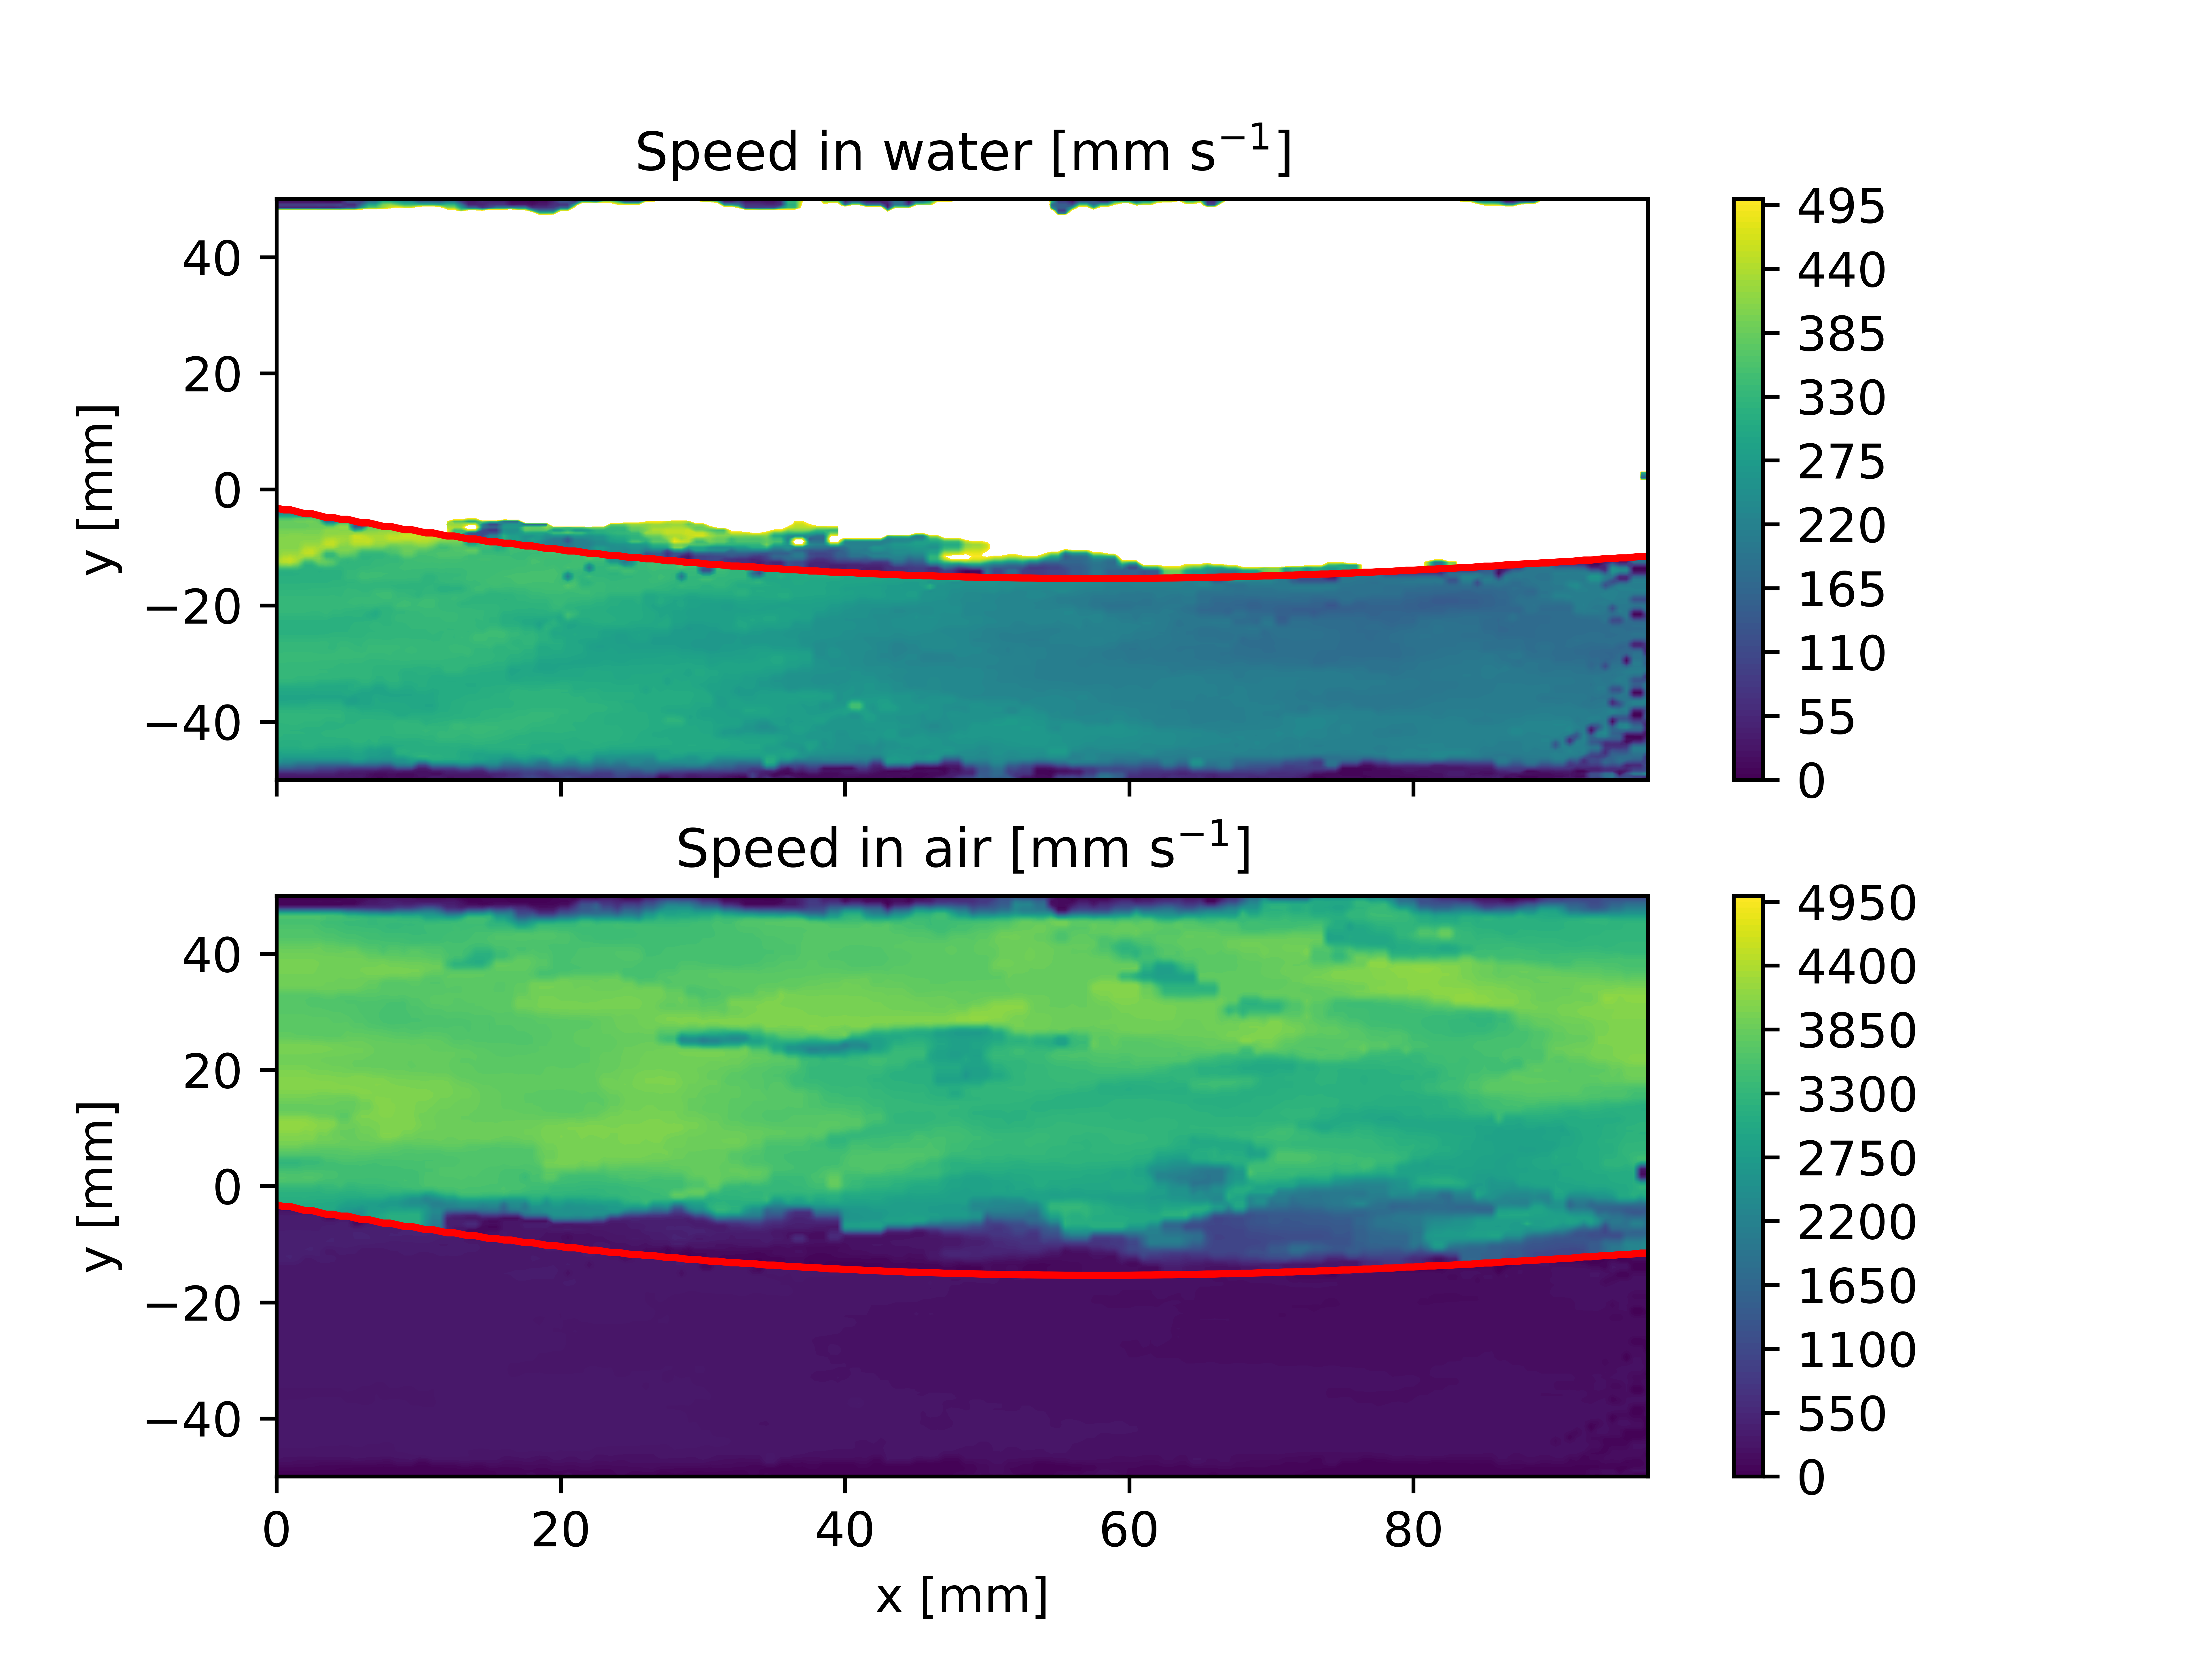
\includegraphics[scale=0.65]{../figures/task_b.png}
    \caption{Contour plot of $\sqrt{u^2 + v^2}$. Red line indicating border between gas and liquid.}
    \label{fig:contour_b}
\end{figure}

\begin{figure}[h!]
    \centering
    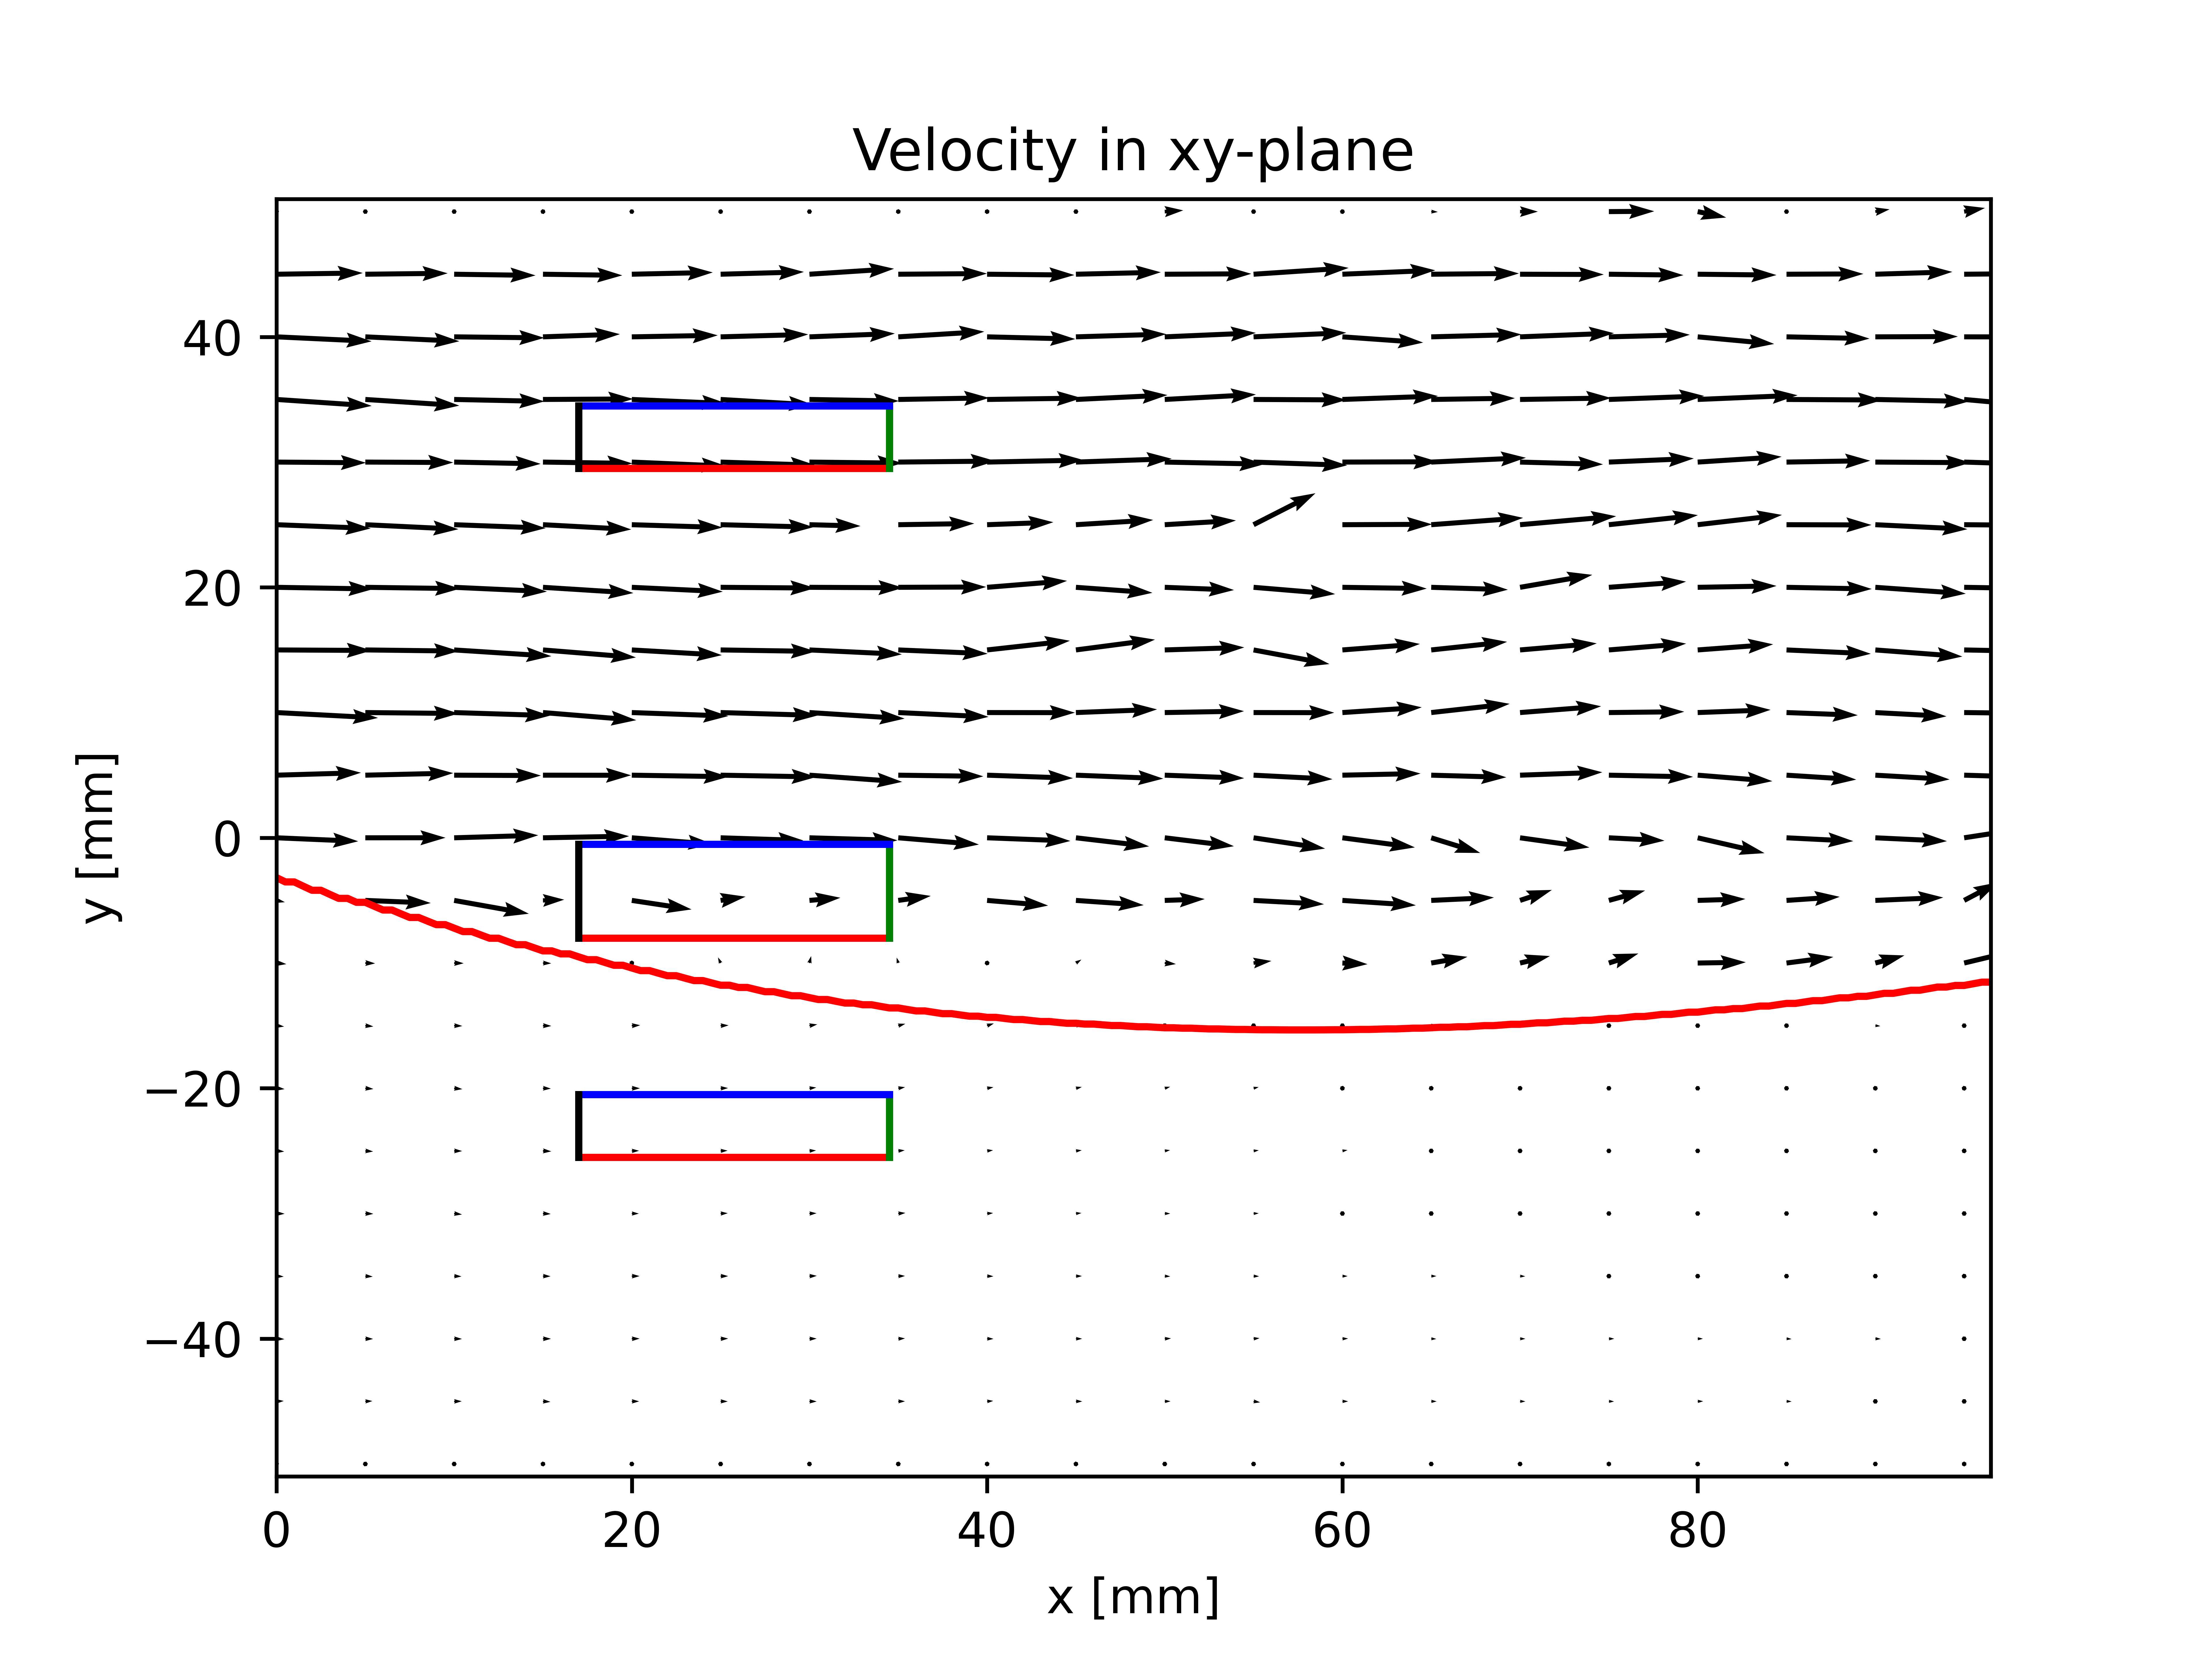
\includegraphics[scale=0.65]{../figures/task_c.png}
    \caption{Quiver plot of velocity $u\bm{i} + v\bm{j}$. Red line indicating border between gas and liquid.}
    \label{fig:quiver_c}
\end{figure}

\newpage
\begin{figure}[h!]
    \centering
    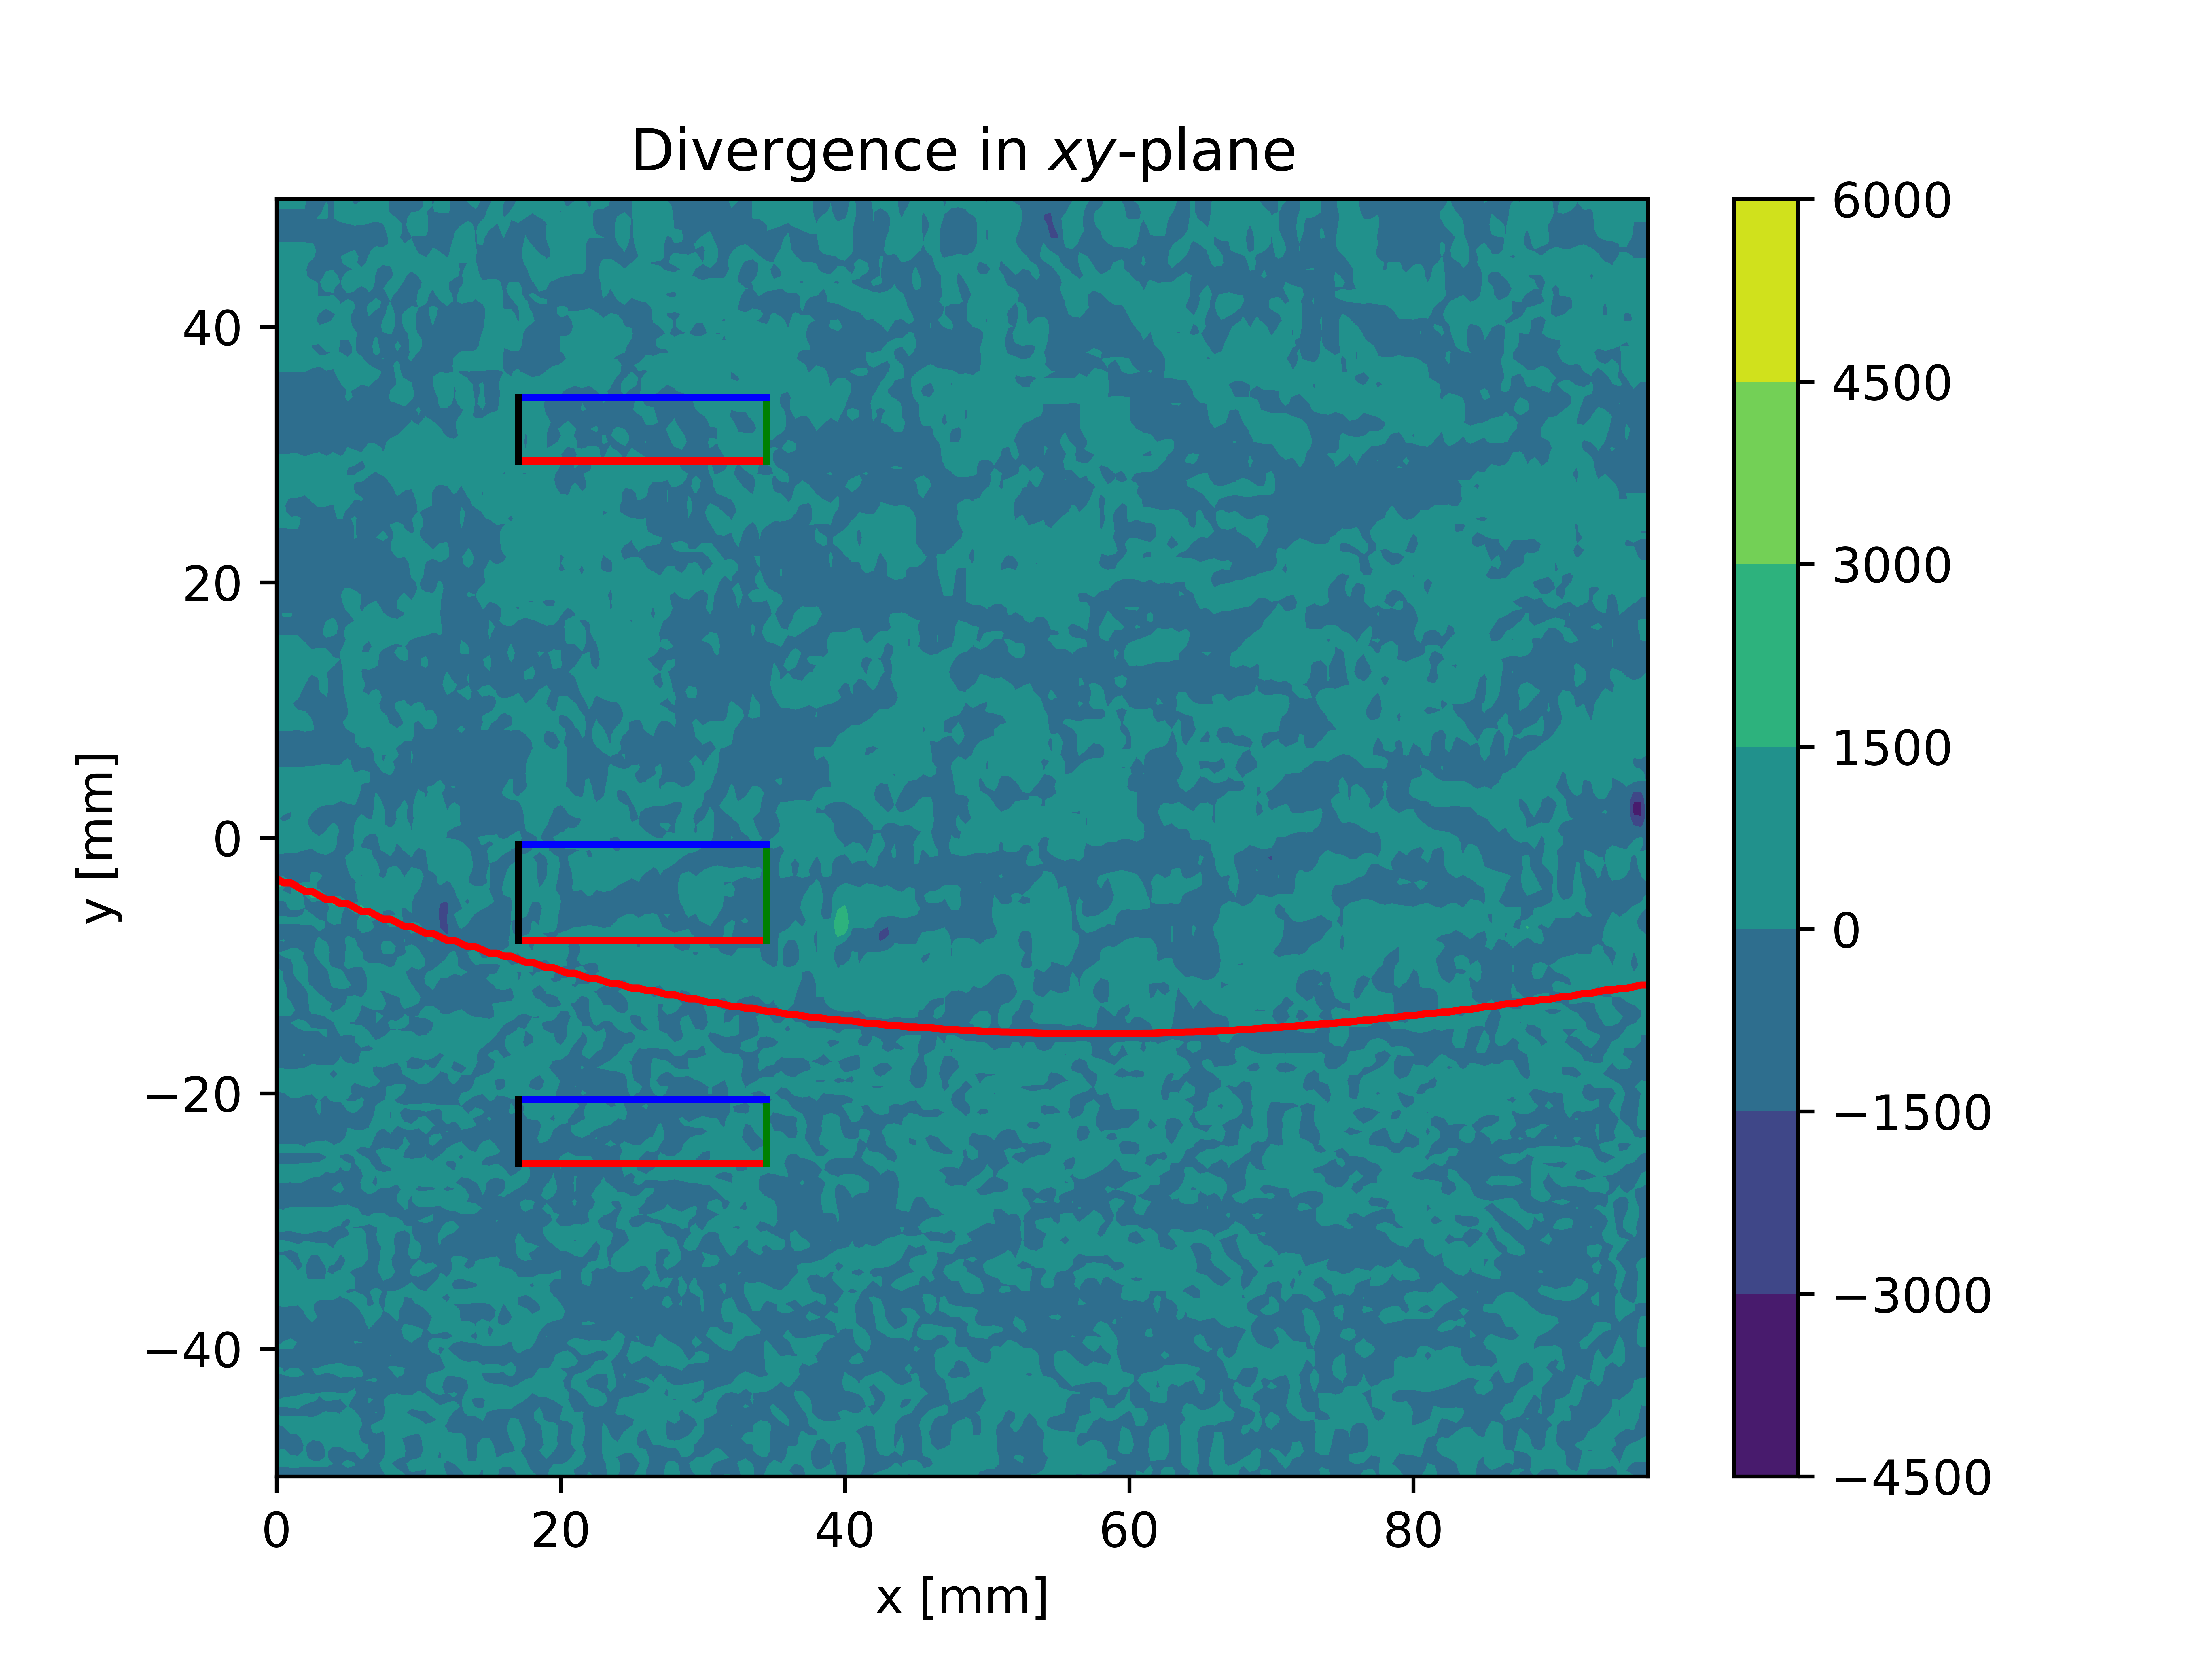
\includegraphics[scale=0.65]{../figures/task_d.png}
    \caption{Contour plot of $\nabla \cdot \bm{v}^*$. Red line indicating border between gas and liquid.}
    \label{fig:contour_d}
\end{figure}

Let $\bm{v} = u\bm{i} + v\bm{j} + w\bm{k}$ and $\bm{v}^* = u\bm{i} + v\bm{j}$. The divergence is
\begin{align*}
    \mathbf{\nabla} \cdot \bm{v}^*
    &= \frac{\partial u}{\partial x} + \frac{\partial v}{\partial y} \\
    \mathbf{\nabla} \cdot \bm{v}
    &= \frac{\partial u}{\partial x} + \frac{\partial v}{\partial y} + \frac{\partial w}{\partial z}
    = \mathbf{\nabla} \cdot \bm{v}^* + \frac{\partial w}{\partial z}
\end{align*}

Since both the gas and the liquid are modeled as incompressible fluids, the divergence should be zero. This means that 
\begin{align*}
    \mathbf{\nabla} \cdot \bm{v}^* + \frac{\partial w}{\partial z} = 0 &
    \implies \frac{\partial w}{\partial z}
    = - \mathbf{\nabla} \cdot \bm{v}^*
\end{align*}

\begin{figure}[h!]
    \centering
    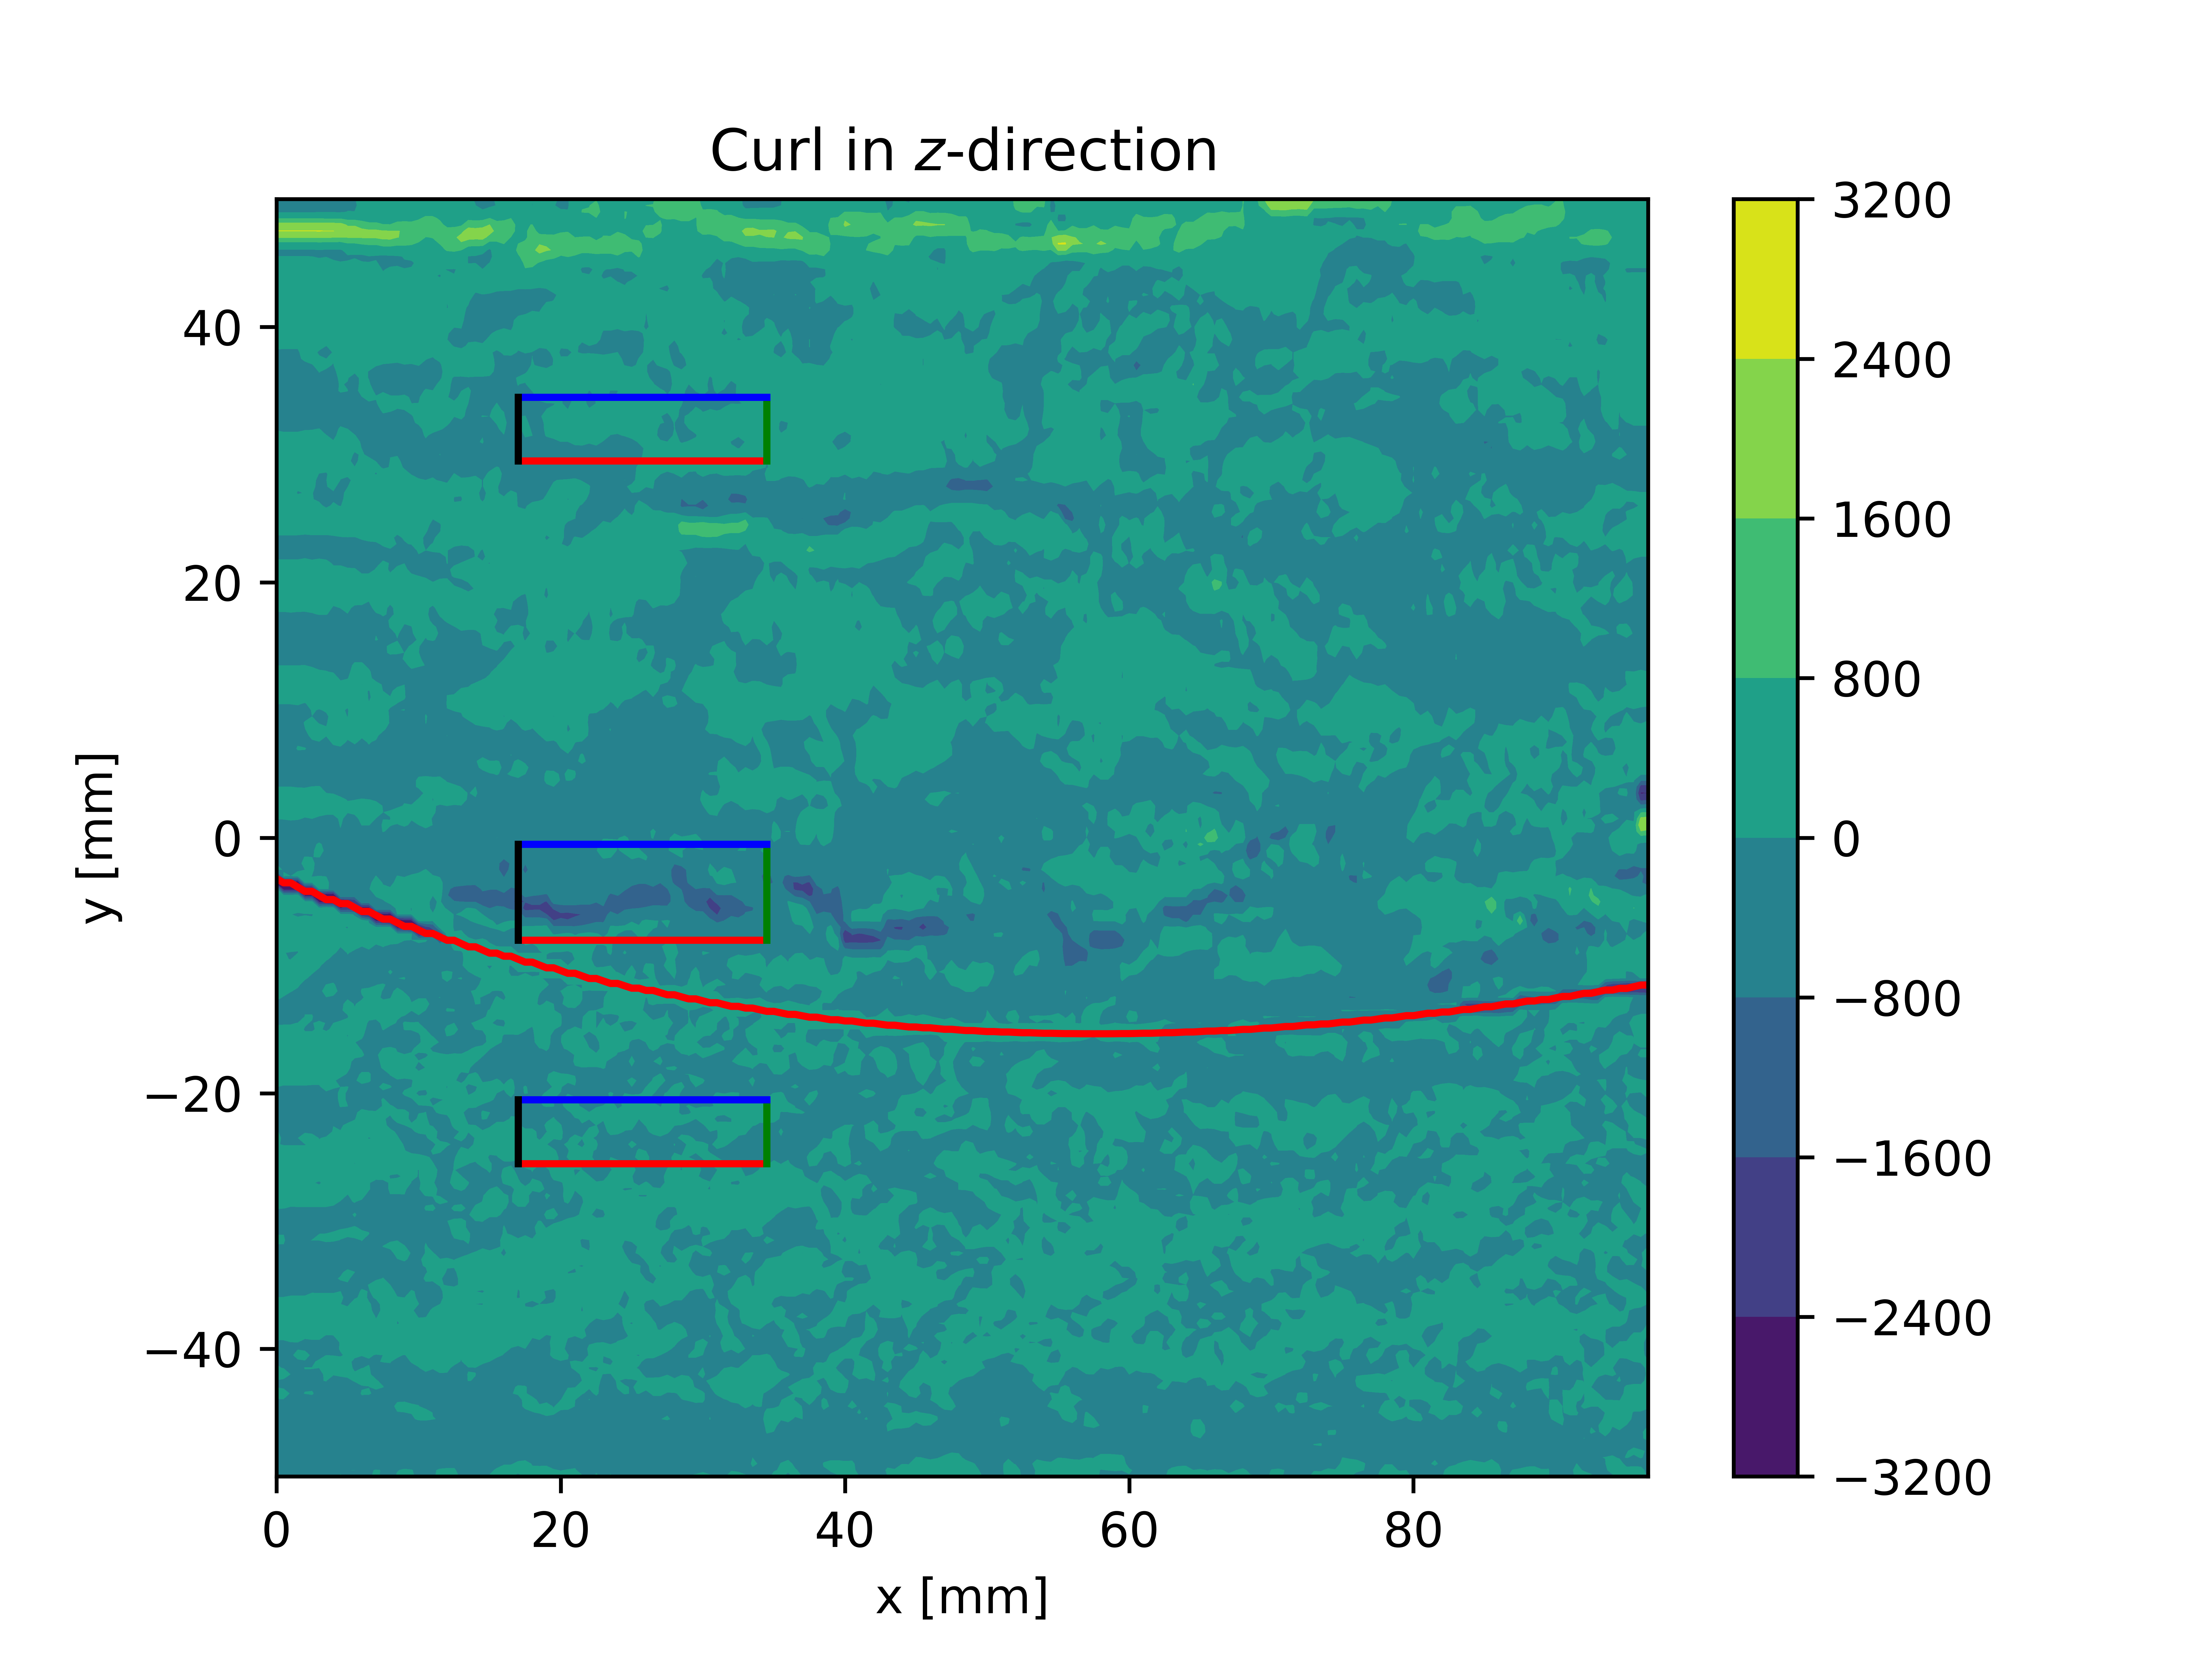
\includegraphics[scale=0.65]{../figures/task_e_curl.png}
    \caption{Contour plot of $(\nabla \times \bm{v}^*) \cdot \bm{k}$. Red line indicating border between gas and liquid.}
    \label{fig:contour_curl}
\end{figure}

From figure \ref{fig:streamlines} we observe that the streamlines mostly follows the expected flow of an irrotational field. There are some deviations at the air-water border, but the curl is still around zero in this area (seen in figure \ref{fig:contour_curl}). At the borders we observe that the flow is not straight. This is due to the friction force between the fuilds and the walls. 

\begin{figure}[h!]
    \centering
    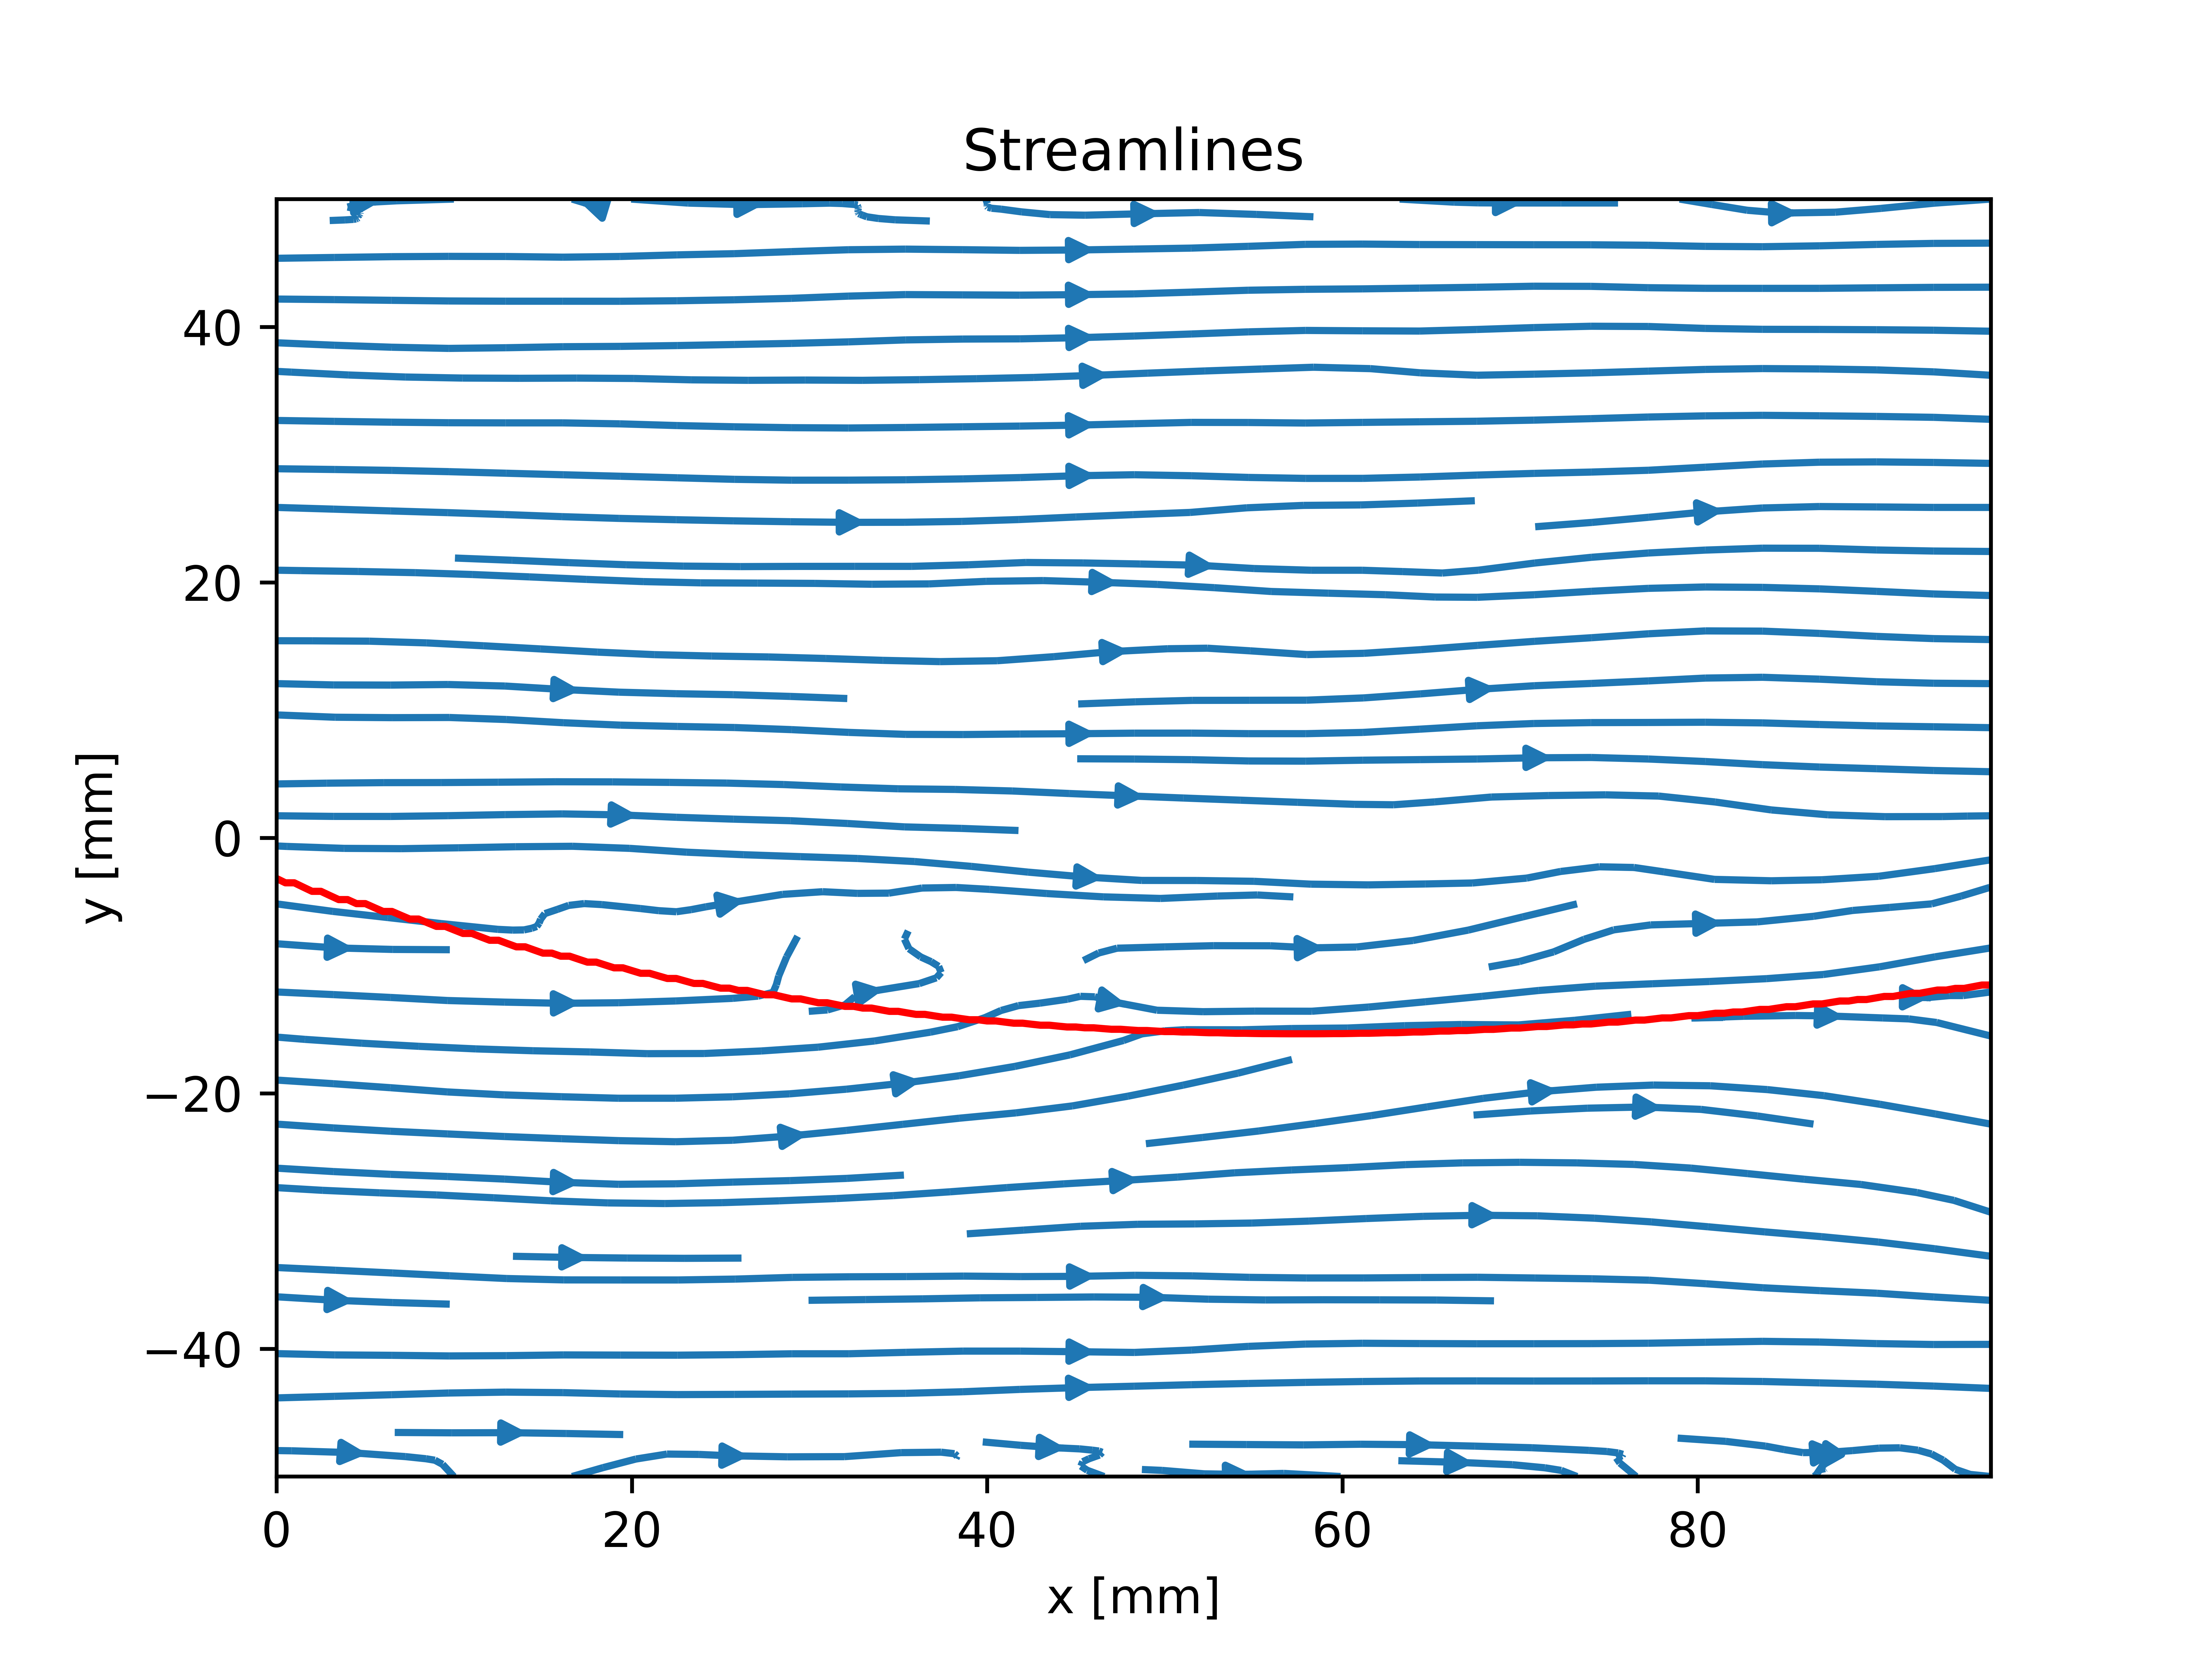
\includegraphics[scale=0.65]{../figures/task_e_streamlines.png}
    \caption{streamlines for $\bm{v}^*$. Red line indicating border between gas and liquid.}
    \label{fig:streamlines}
\end{figure}

\newpage
The code in $\verb|integration.py|$ yields the following result:
\lstinputlisting[numbers=none]{../integration_out.txt}

For the rectangles in the part of the field located in the air, the difference between the line integral and the surface integral is negligible. For all three rectangles, the circulation is a lot larger in x direction, as expected. The values for the circulation around each side of the rectangles are as expected, with larger values where the velocity is higher. For the rectangle located in the water (rectangle 3), the difference between the line integral and the surface integral is very large, yet both values are a lot smaller than rectangle 1 and 2, since the velocity is a lot lower in the water. The error is likely due to our limited resolution ($\Delta x = \Delta y = 0.5$mm).

The divergence theorem states
\begin{align*}
    \oint_C \bm{F} \cdot d\bm{s}
    = \int_V \bm{\nabla} \cdot \bm{F} dV
\end{align*}

Remembering that the fluid is incompressible, yet having $\bm{\nabla} \cdot \bm{v}^* \neq 0$ results in the surface integral $\int_{\sigma} \bm{\nabla} \cdot \bm{v}^* d\sigma \neq 0$. This means that the integrated flux in z direction for $\bm{v}$ would be $-\int_{\sigma} \bm{\nabla} \cdot \bm{v}^* d\sigma$ to ensure that $\int_{\sigma} \bm{\nabla}\cdot \bm{v} d\sigma = 0$.

For all three rectangles we observe that the integrated flux is a large positive value for side number two and a large negative value for side number four. This is reasonable as there is a lot of flow in through the left side and out through the right. Rectangle 2 has a large negative integrated flux due to its placement close to the separation surface between water and air.

\newpage
File: $\verb|plots.py|$
\lstinputlisting{../plots.py}

File: $\verb|integration.py|$
\lstinputlisting{../integration.py}

\end{document}
